\documentclass{article}
\usepackage[utf8]{inputenc}
\usepackage{caption}
\usepackage{graphicx}
\usepackage{listings}
\usepackage{amsmath}
\usepackage[framed,numbered,autolinebreaks,useliterate]{mcode}

\title{ENGN4528 Computer Vision Clab2 Report}
\author{Zhipeng Bao ~~ u6600985}
\date{March 2018}

\begin{document}

\maketitle

\section*{Task 1: Implement your own Harris Corner Detector}
\subsubsection*{Step 1 \& Step 2: Read, understand and Complete the Matlab codes.}
For this task, we are required to finish the Harris Corner Detector based on the existing codes. From the lecture, we know that there are two main process in the Harris Corner detection algorithm: \emph{Find the points with large corner response function R} and \emph{Find the local maximum value of the response}. By reading the half-finished codes, I found that the missing parts are exactly the two main process.

For the first part, we need to get the function $R$ which equals:

\begin{equation}
    R = det(M)-k*(trace(M))^2
\end{equation}

In the equation, k is a constant value varies from 0.04 to 0.06. We set it as a most widely used value: 0.04. And the matrix $S$ has the following defination:

\[
\centering
\begin{bmatrix}
    \sum (I_x(x,y))^2 & \sum I_x(x,y)I_y(x,y) \\
    \sum I_x(x,y)I_y(x,y) & \sum (I_y(x,y))^2
\end{bmatrix}
\]

For the next main process, we need to find the local maximum which can be calculated by Matlab inbuilt function ordfit2(). Then we need to find the ones that are larger than threshold.

I made a lot of comments in my codes. So step 3 shows the details of the whole process.

\subsubsection*{Step 3: Comment on the codes.}
The codes and the comments are shown below:

\begin{lstlisting}
function [rws,cols] = my_corner_detector(bw, sig, thre,sz)
    %Harris Corner Detector
    % parameters
    sigma = sig;
    thresh = thre;
    sze = sz;
    disp = 0;
    
    bw = double(bw); %transform image to double
    [line,column] = size(bw);%get the size
    
    dy = [-1 0 1; -1 0 1; -1 0 1]; % derivative mask in y direction
    dx = dy'; % dx and dy have symmetrical structure

    % image derivatives
    Ix = conv2(bw,dx,'same'); % derivatives in x direction
    Iy = conv2(bw,dy,'same'); % derivatives in y direction


    %need codes here
    g = fspecial('gaussian',max(1,fix(6*sigma)),sigma); % form a gaussian kernel
    Ix2 = conv2(Ix.^2,g,'same');%Smoothed image derivatives and calculate M(1,1)
    Iy2 = conv2(Iy.^2,g,'same'); %calculate M(1,2) and M(2,1)
    Ixy = conv2(Ix.*Iy,g,'same'); %calculate M(2,2)

    Ix2 = padarray(Ix2, [(sze-1)/2, (sze-1)/2]); %make it convinient for later work
    Iy2 = padarray(Iy2, [(sze-1)/2, (sze-1)/2]); %make it convinient for later work
    Ixy = padarray(Ixy, [(sze-1)/2, (sze-1)/2]); %make it convinient for later work

    %compute the cornerness
    k = 0.04; % range of k: 0.04~0.06, 0.04 is a widely used value for Haris Detector
    
    for i = 1:line
        for j=1:column
            xx = sum(sum(Ix2(i:i+sze-1,j:j+sze-1))); %calculate sum of Ix^2
            yy = sum(sum(Iy2(i:i+sze-1,j:j+sze-1))); %calculate sum of Iy^2
            xy = sum(sum(Ixy(i:i+sze-1,j:j+sze-1))); %calculate sum of Ixy
            M = [xx,xy;xy,yy]; %represent M
            cornerness(i,j) = det(M)-k*trace(M)^2; %calculate det(M) - k*trace(M)^2, which is the cornerness
        end
    end

    max_value = ordfilt2(double(cornerness), sze^2, ones(sze)); %find local maximum points

    cornerness = (double(cornerness) == max_value) & (double(cornerness) > thresh); %find local max points and the ones bigger than thresh
    [rws, cols] = find(cornerness>0); %get result
end


\end{lstlisting}

\subsubsection*{Step 4 - Step 6: Display and compare the results.}

Fig 1 shows the result on lenna with different threshold. We can see that the corners get fewer with a bigger threshold. And the sharper corners left with the bigger threshold.

\begin{figure}[htbp]
    \centering
    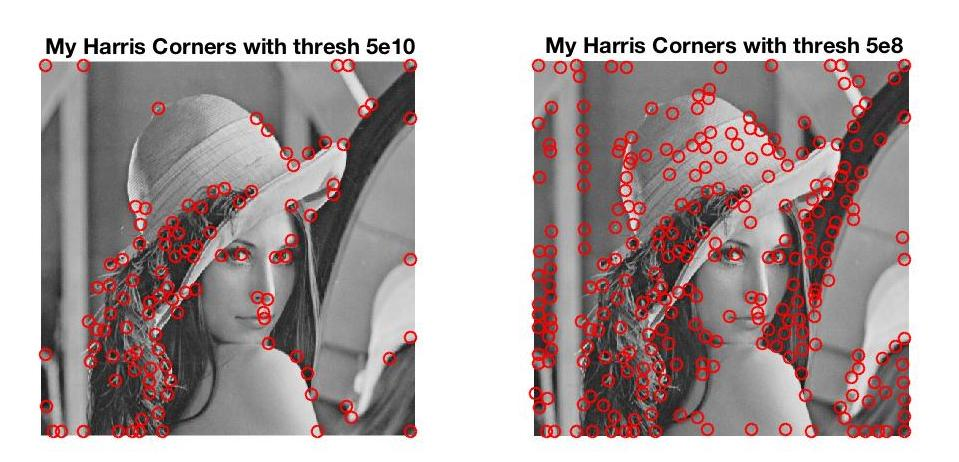
\includegraphics[scale = 0.25]{fig1.jpg}
    \caption{Result for Lenna with different threshold}
    \label{fig1}
\end{figure}

Figure 2 to figure 5 show the results with $thresh = 5e10$ and compare them with Matlab inbuilt corner functions. We can see there are some different points between my function and Matlab inbuilt function. I think the reason is that the threshold and sigma are different. Besides, the inbuilt function may also use some optimal methods.
\begin{figure}[htbp]
    \centering
    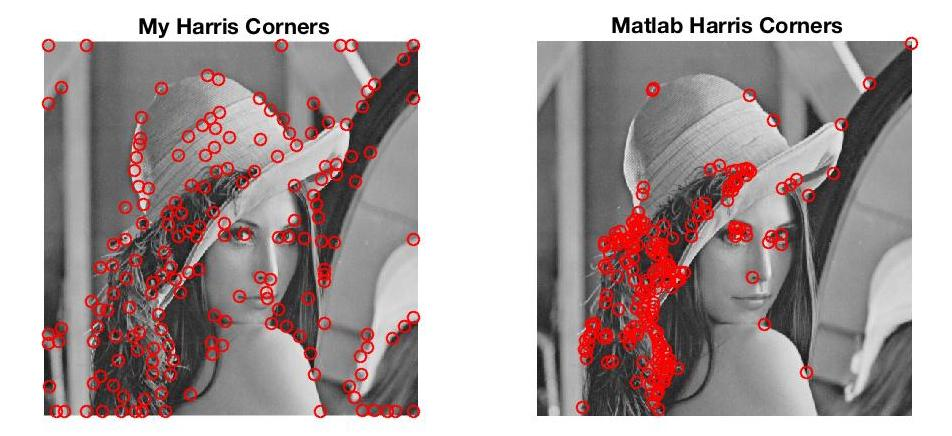
\includegraphics[scale = 0.25]{fig2.jpg}
    \caption{}
    \label{fig2}
\end{figure}
\begin{figure}[htbp]
    \centering
    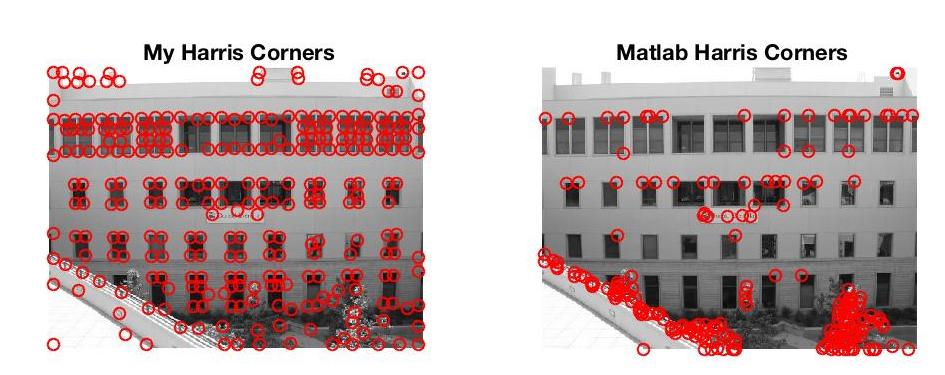
\includegraphics[scale = 0.25]{fig3.jpg}
    \caption{}
    \label{fig3}
\end{figure}
\begin{figure}[htbp]
    \centering
    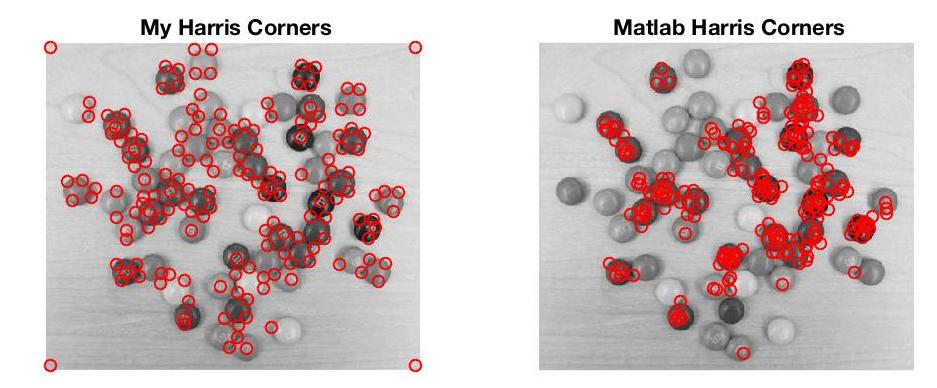
\includegraphics[scale = 0.25]{fig4.jpg}
    \caption{}
    \label{fig4}
\end{figure}
\begin{figure}[htbp]
    \centering
    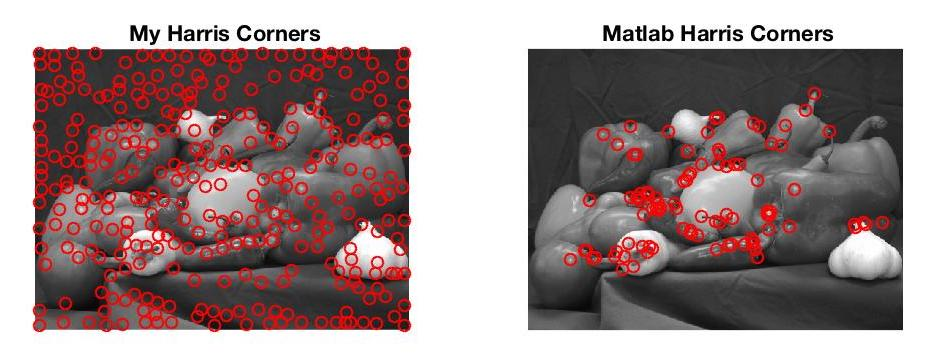
\includegraphics[scale = 0.25]{fig5.jpg}
    \caption{}
    \label{fig5}
\end{figure}

\section*{Taks 2: Implement your own k-means clustering function, and use it for colour image segmentation}

\subsubsection*{Step 1 \& Step 2: Read in and convert the image.}

The codes for the first three steps are given. The only difference is for the uint 16 image. The codes are in the following.

\begin{lstlisting}
    %Step 1: Read input image
    path1 = './images/Peppers.png';
    img1 = imread(path1);
    img1 = uint8(img1/2^8);
    imshow(img1);
\end{lstlisting}

\subsubsection*{Step 3: Form 5-dimensional feature vector. }

I checked the given codes for this problem. It is correct.

\subsubsection*{Step 4 : Implement your own k-means algorithm.}

First, the given half-finished codes have one mistake. In the $17^{th}$ line, the codes should be:
\begin{lstlisting}
    %distances = zeros(ndata,ndims); wrong!
    distances = zeros(ndata,nc); % right
\end{lstlisting}

Then there are two parts of codes that I need to fulfill. The first thing is to assign each point to the nearest cluster center. The second is to update the membership assignment. Actually, these two thing is a whole part. I divide it into another two parts: Calculate the distance between each point and each cluster center. The missing codes are in the following:

\begin{lstlisting}
    % - calculate the distance from each point to each cluster center.  
    cluster_position = cluster_stats(:,2:end); 
    for i = 1:nc
        a = data-repmat(cluster_position(i,:),ndata,1);
        distances(:,i) = sqrt(sum(a.^2,2));
    end
    
	%%update the membership assignment, i.e., update the data_clusters with current values.  
    for i = 1:ndata
        data_clusters(i) = find(distances(i,:) == min(distances(i,:)),1);
    end
\end{lstlisting}

\subsubsection*{Step 5: Display the results.}
For the result of my k-mean algorithm, I firstly set k to 5. The result with different factor for different images are shown in Figure 6 to Figure 15.

\begin{figure}[htbp]
    \centering
    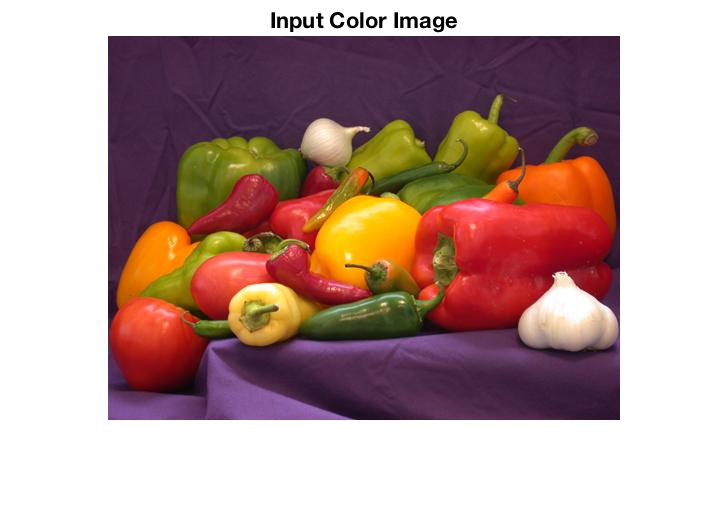
\includegraphics[scale = 0.25]{fig6.jpg}
    \caption{The first color image.}
    \label{fig6}
\end{figure}\begin{figure}[htbp]
    \centering
    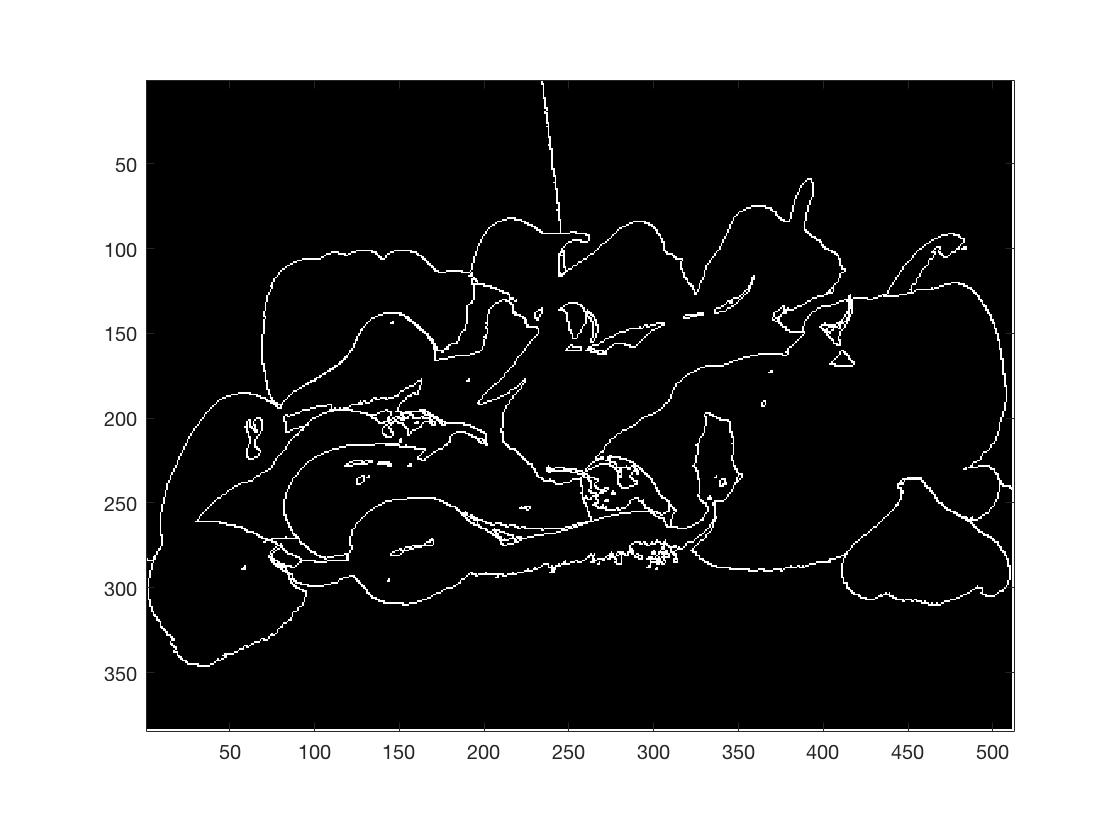
\includegraphics[scale = 0.25]{fig8.jpg}
    \caption{The boudnary of the first image.}
    \label{fig7}
\end{figure}
\begin{figure}[htbp]
    \centering
    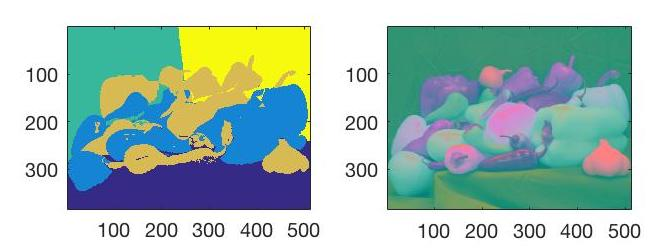
\includegraphics[scale = 0.4]{fig7.jpg}
    \caption{The 5-means result with factor = 1}
    \label{fig8}
\end{figure}

\begin{figure}[htbp]
    \centering
    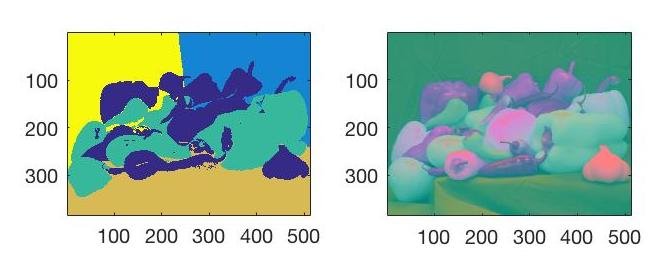
\includegraphics[scale = 0.4]{fig9.jpg}
    \caption{The 5-means result with factor = 0.1}
    \label{fig9}
\end{figure}

\begin{figure}[htbp]
    \centering
    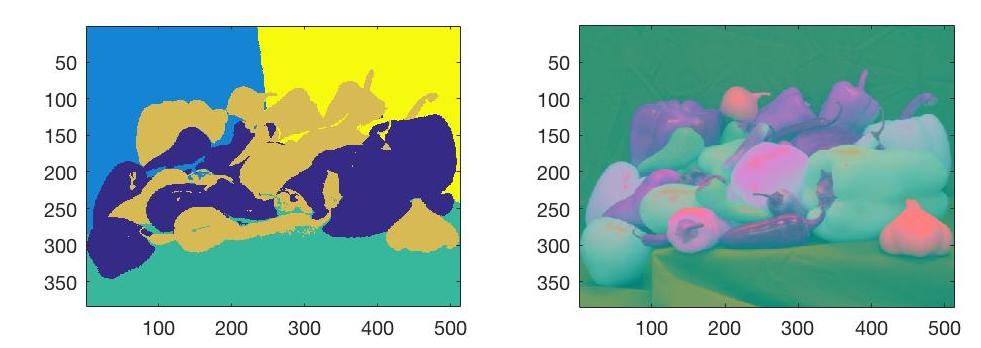
\includegraphics[scale = 0.25]{fig10.jpg}
    \caption{The 5-means result with factor = 10}
    \label{fig10}
\end{figure}

\begin{figure}[htbp]
    \centering
    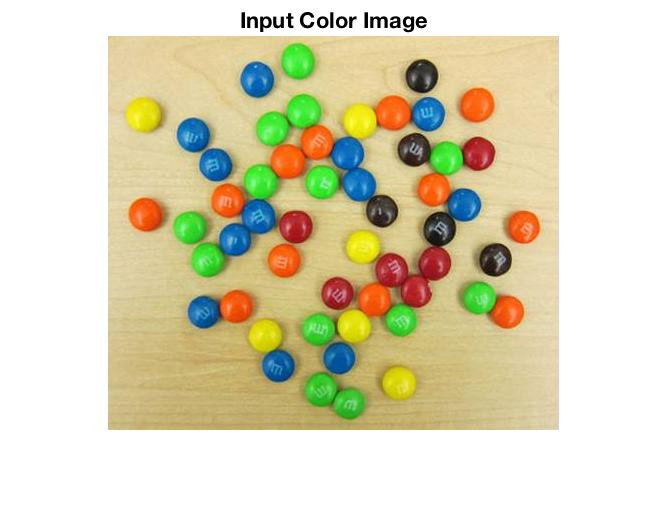
\includegraphics[scale = 0.25]{fig11.jpg}
    \caption{The second image.}
    \label{fig11}
\end{figure}

\begin{figure}[htbp]
    \centering
    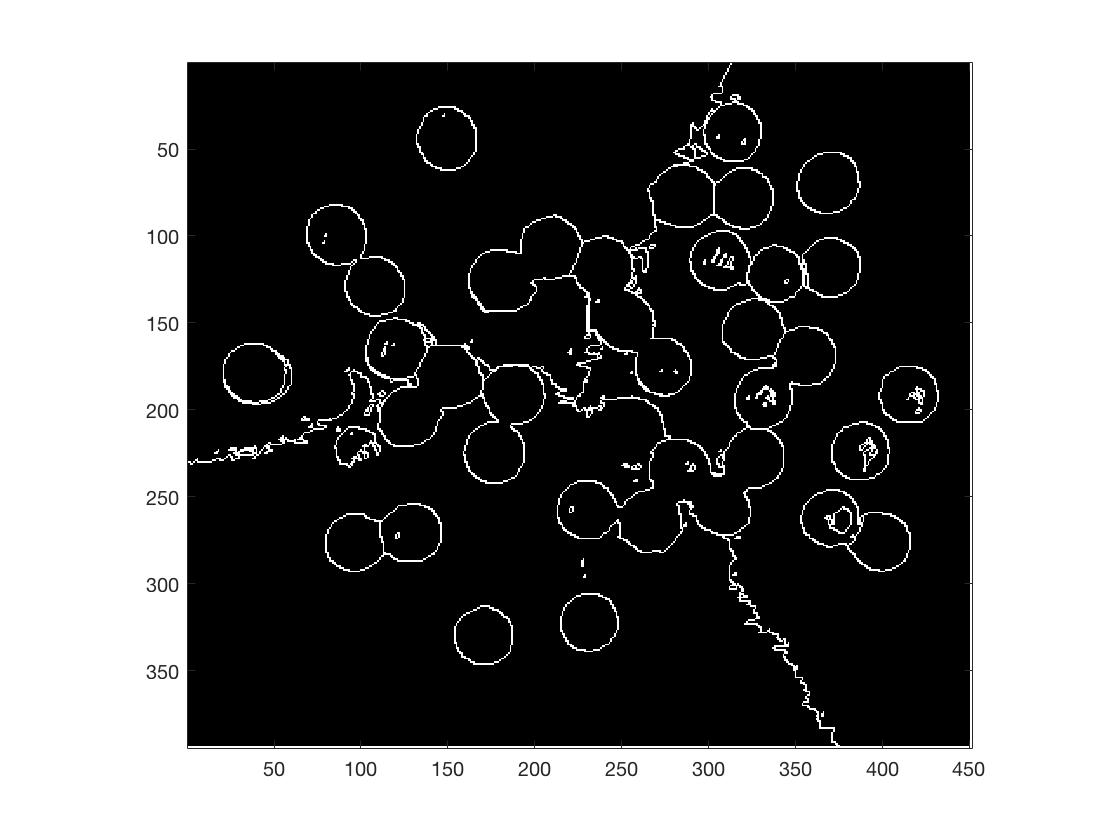
\includegraphics[scale = 0.25]{fig13.jpg}
    \caption{The boudnary of the second image}
    \label{fig12}
\end{figure}

\begin{figure}[htbp]
    \centering
    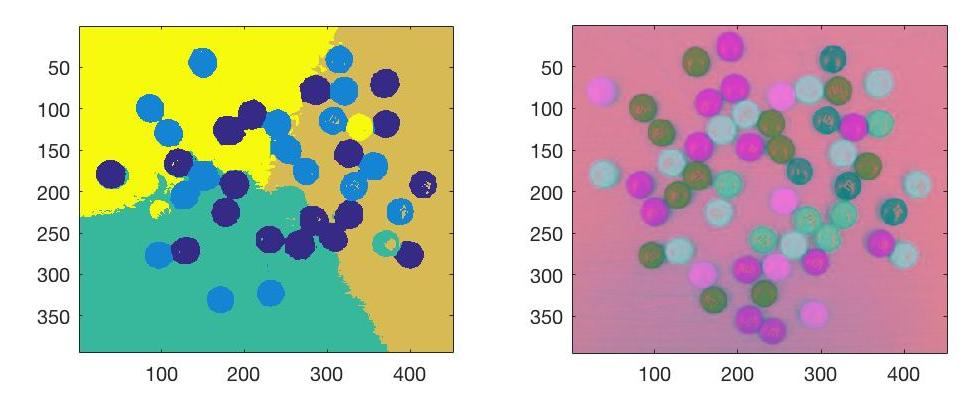
\includegraphics[scale = 0.25]{fig12.jpg}
    \caption{The 5-means result with factor = 1}
    \label{fig13}
\end{figure}

\begin{figure}[htbp]
    \centering
    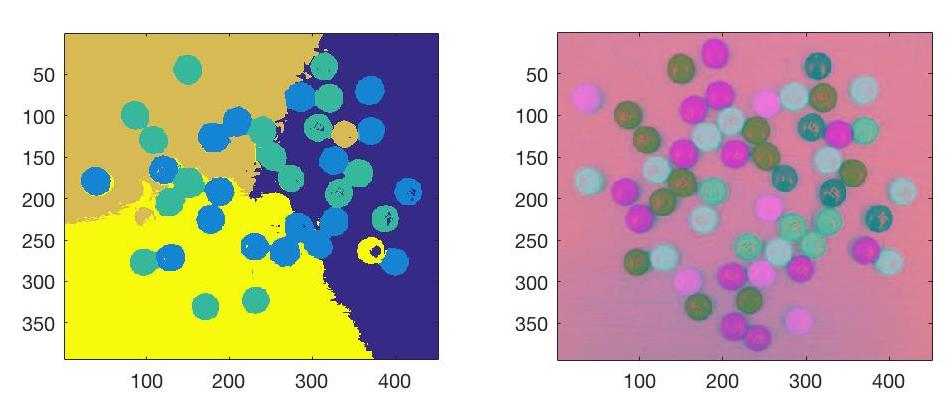
\includegraphics[scale = 0.25]{fig14.jpg}
    \caption{The 5-means result with factor = 10}
    \label{fig14}
\end{figure}

\begin{figure}[htbp]
    \centering
    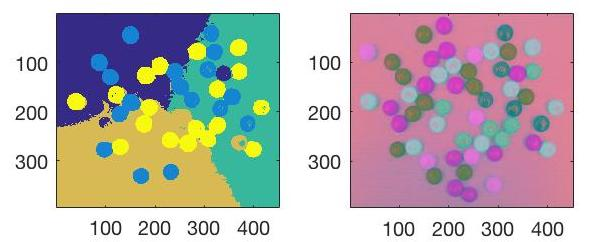
\includegraphics[scale = 0.4]{fig15.jpg}
    \caption{The 5-means result with factor = 0.1}
    \label{fig15}
\end{figure}

From the result I found no difference among the different factors. However, I read the codes carefully and think about the function of the factor. In my opinion, the factor is used to times coordinates of each feature vector, and make the values bigger than before. When using a bigger factor, more values will be set as maximum, then the boundary will be influenced. 

I think maybe the reason is that the number of the classes is too small to show the difference. So I change the k to 10 and redo the experiment.

The result of the MMS are shown as follows:
\begin{figure}[htbp]
    \centering
    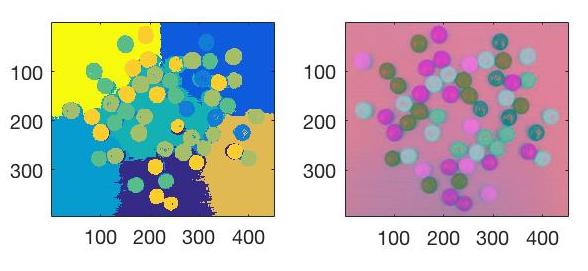
\includegraphics[scale = 0.4]{fig16_10.jpg}
    \caption{The 10-means result with factor = 10}
    \label{fig16}
\end{figure}

\begin{figure}[htbp]
    \centering
    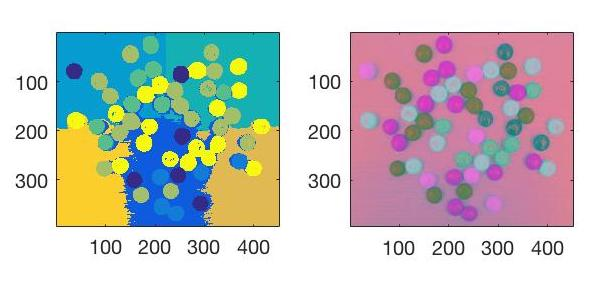
\includegraphics[scale = 0.4]{fig17.jpg}
    \caption{The 10-means result with factor = 0.1}
    \label{fig17}
\end{figure}

This time, we can see the clear difference between different factor. It also prove my assumption of the factor.


\section*{Task 3: Play with SIFT code, and implement an image match algorithm}

\subsubsection*{Step 1: Read in image and rotate it.}
This task is quite simple. Here I show the results. The codes can be found in the next part (attached codes.)

\begin{figure}[htbp]
    \centering
    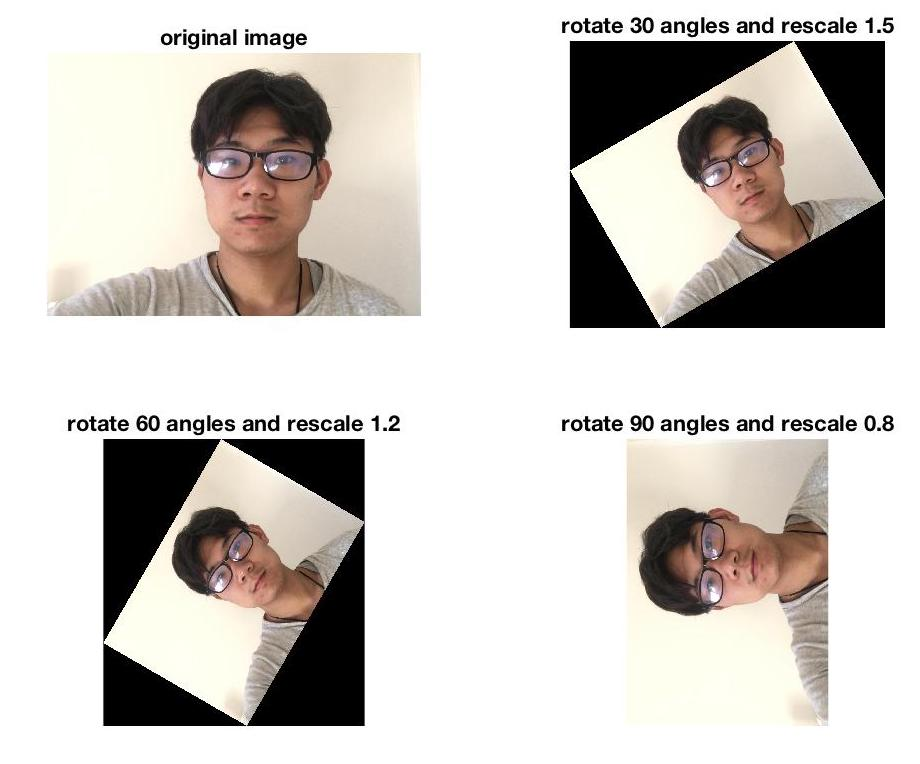
\includegraphics[scale = 0.3]{fig18.jpg}
    \caption{The original images and rotated and rescaled images.}
    \label{fig18}
\end{figure}

\subsubsection*{Step 2: Read, understand and test SIFT function.}

I read the codes of $sift.m$ carefully and understand how it works. The first step is to restore the file in a pgm form. Then, use external sift binary file to calculate the sift values (in tmp.key file). The final step is to transform the values to descriptors and locs. The first two dimensions of locs are the column and line number of the points. Then the scale and the ori.

However, although I have two operation systems myself, I cannot run the codes. For my mac system, it shows the binary file cannot be run and for my windows system, win32 file also failed. So I changed the codes a little and use a ubuntu server to finish the sift file. I divide the codes for two parts: use external method to calculate the related features.

The first part of the codes are as follows:

\begin{lstlisting}
    fin = imread('face_02_u6600985.jpg');
    imwrite(fin,'im0.pgm');
\end{lstlisting}

For the second part, I rewrite the function below:
\begin{lstlisting}
function [descriptors, locs] = my_sift(image,keys)
% Summarize and reduce some parts of the given sift function.
% The reason is that my mac cannot do the sift and my windows does not
% support win32.
% Thus I use a ubuntu server to finish sift and this function is used to
% get the sift points.
%
% image: XXX.jpg, original image.
% keys: the XXX.key file got from the sift.
[rows, cols] = size(image); 

% Open tmp.key and check its header.
g = fopen(keys, 'r');
if g == -1
    error('Could not open file tmp.key.');
end
[header, count] = fscanf(g, '%d %d', [1 2]);
if count ~= 2
    error('Invalid keypoint file beginning.');
end
num = header(1);
len = header(2);
if len ~= 128
    error('Keypoint descriptor length invalid (should be 128).');
end

% Creates the two output matrices (use known size for efficiency)
locs = double(zeros(num, 4));
descriptors = double(zeros(num, 128));

% Parse tmp.key
for i = 1:num
    [vector, count] = fscanf(g, '%f %f %f %f', [1 4]); %row col scale ori
    if count ~= 4
        error('Invalid keypoint file format');
    end
    locs(i, :) = vector(1, :);
    
    [descrip, count] = fscanf(g, '%d', [1 len]);
    if (count ~= 128)
        error('Invalid keypoint file value.');
    end
    % Normalize each input vector to unit length
    descrip = descrip / sqrt(sum(descrip.^2));
    descriptors(i, :) = descrip(1, :);
end
fclose(g);

\end{lstlisting}

The following codes are attached in the next part. Figure 19 to Figure 22 show the results of sift functions.

\begin{figure}[htbp]
    \centering
    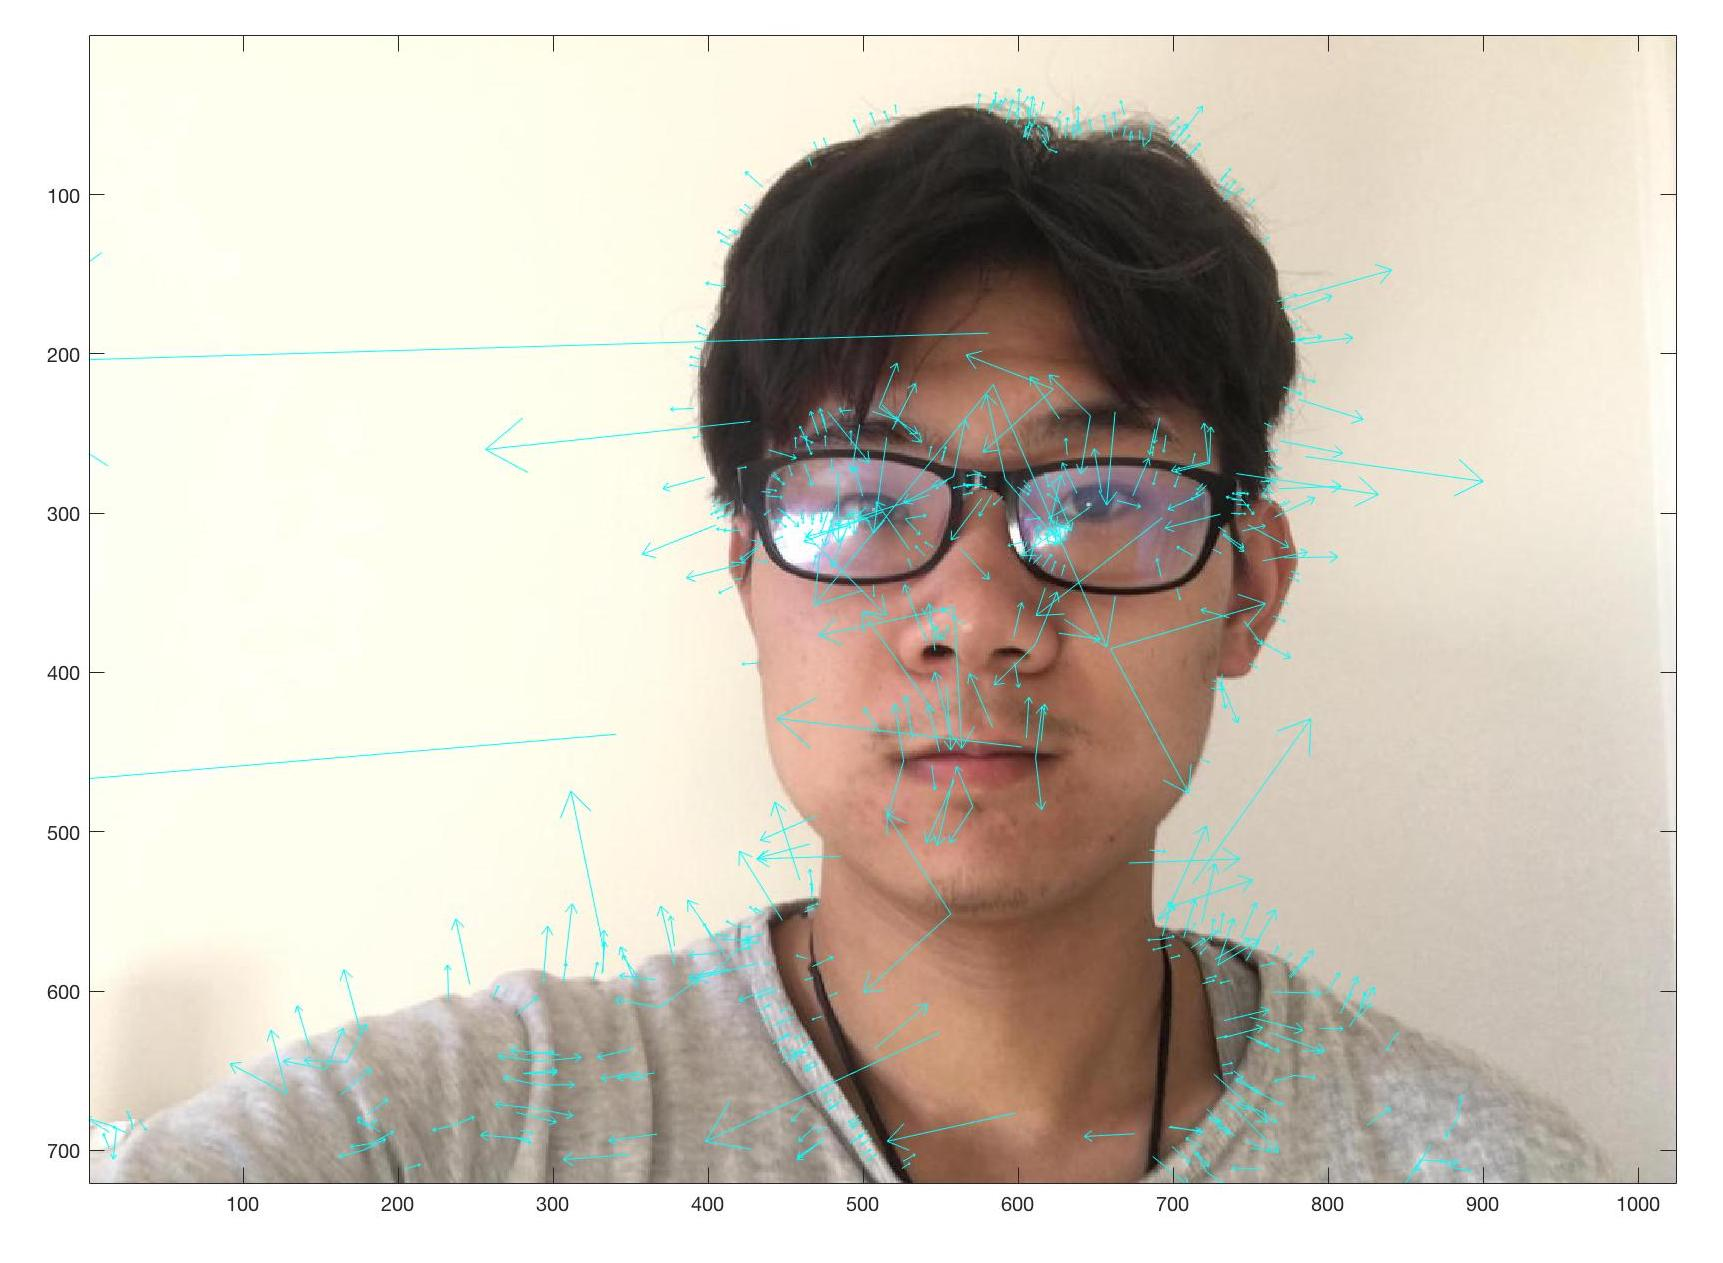
\includegraphics[scale = 0.1]{fig19.jpg}
    \caption{SIFT result of the original image.}
    \label{fig19}
\end{figure}

\begin{figure}[htbp]
    \centering
    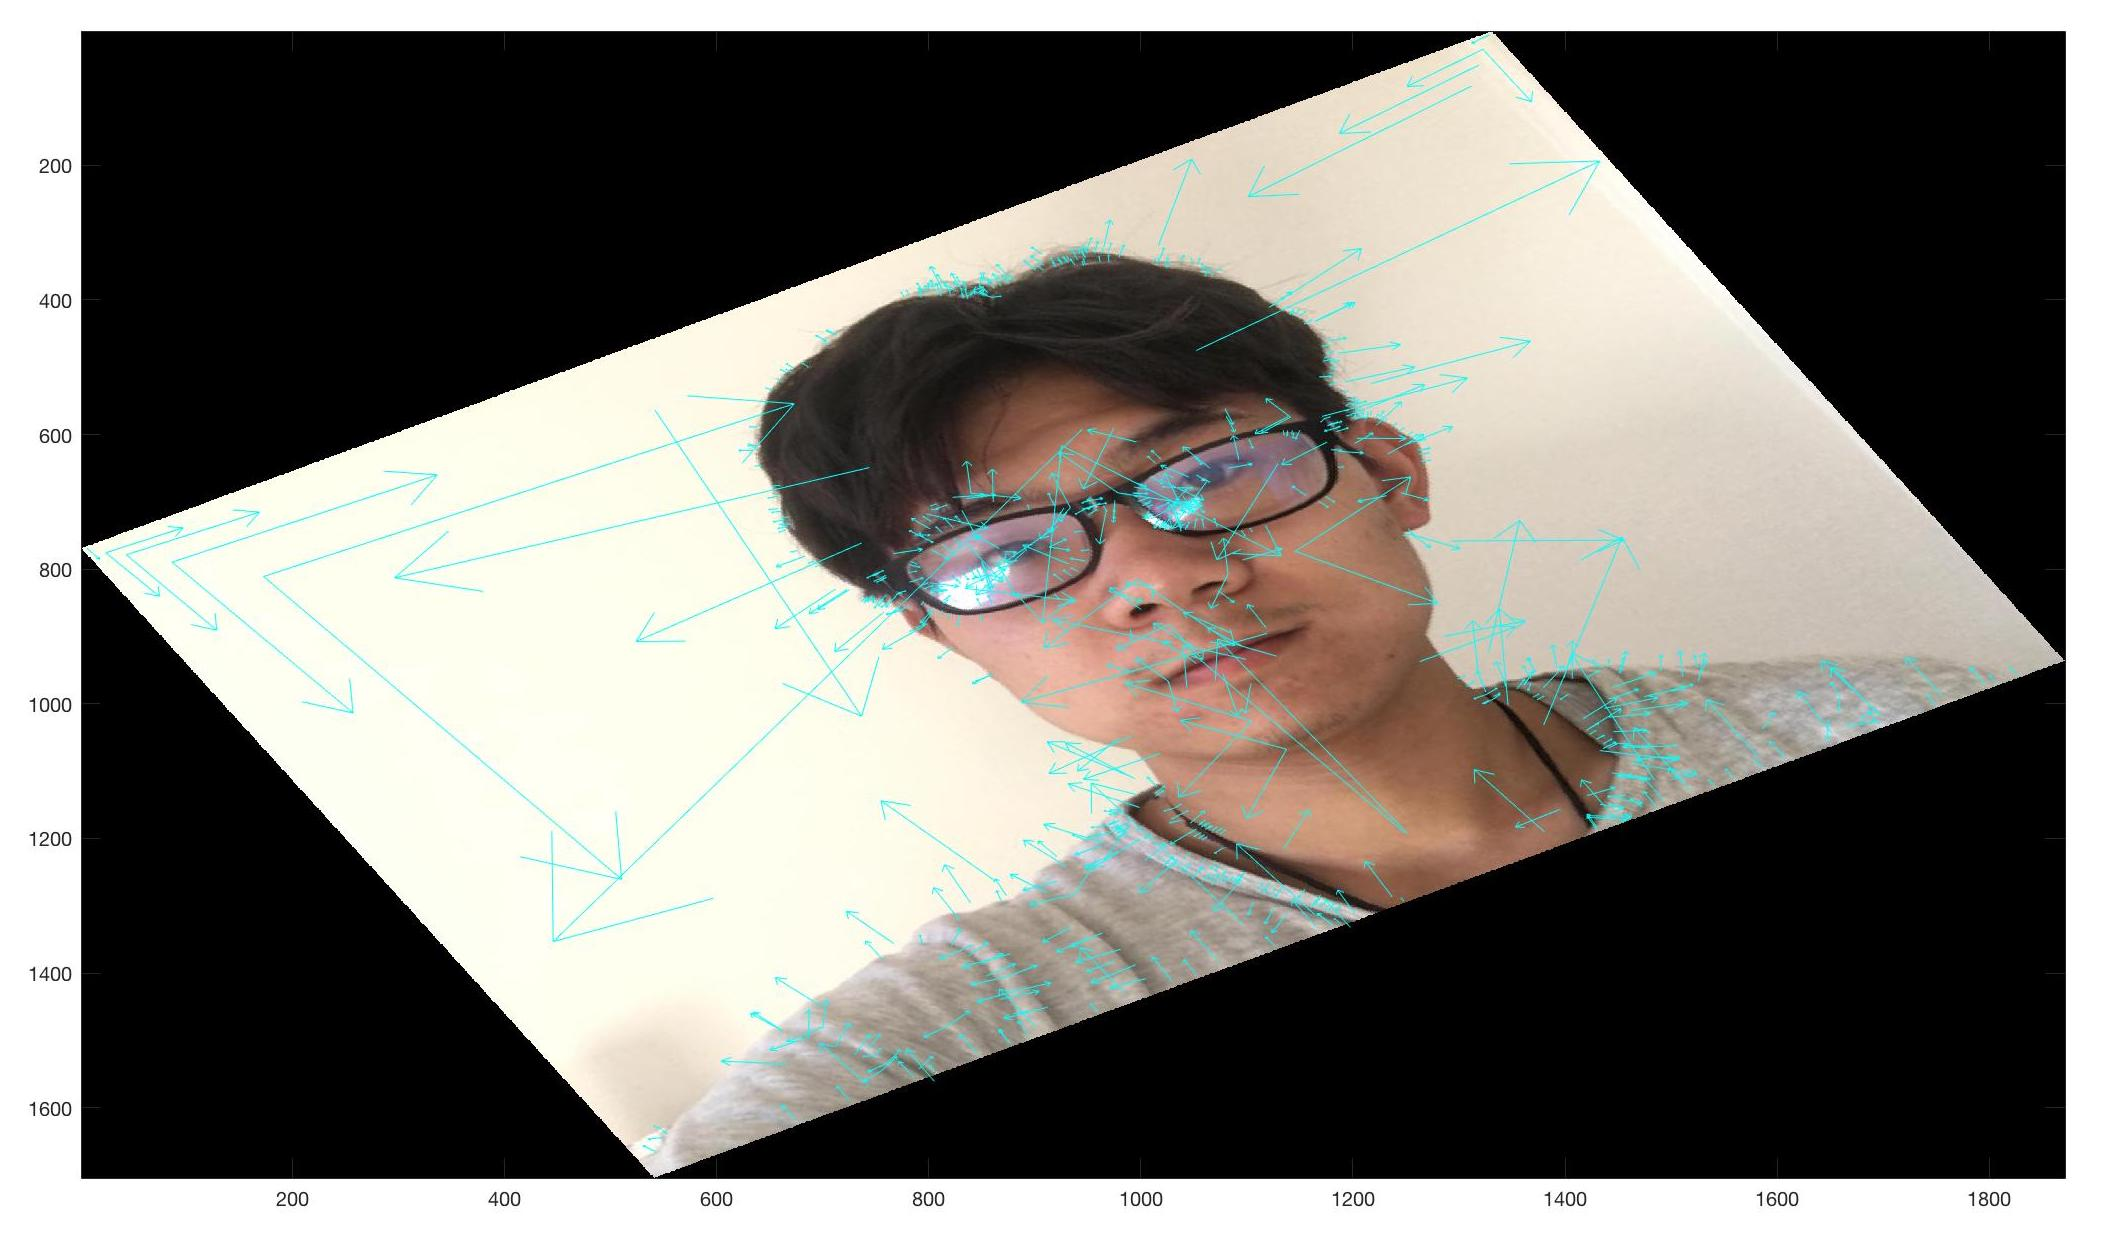
\includegraphics[scale = 0.1]{fig20.jpg}
    \caption{SIFT result of the first processed image.}
    \label{fig20}
\end{figure}

\begin{figure}[htbp]
    \centering
    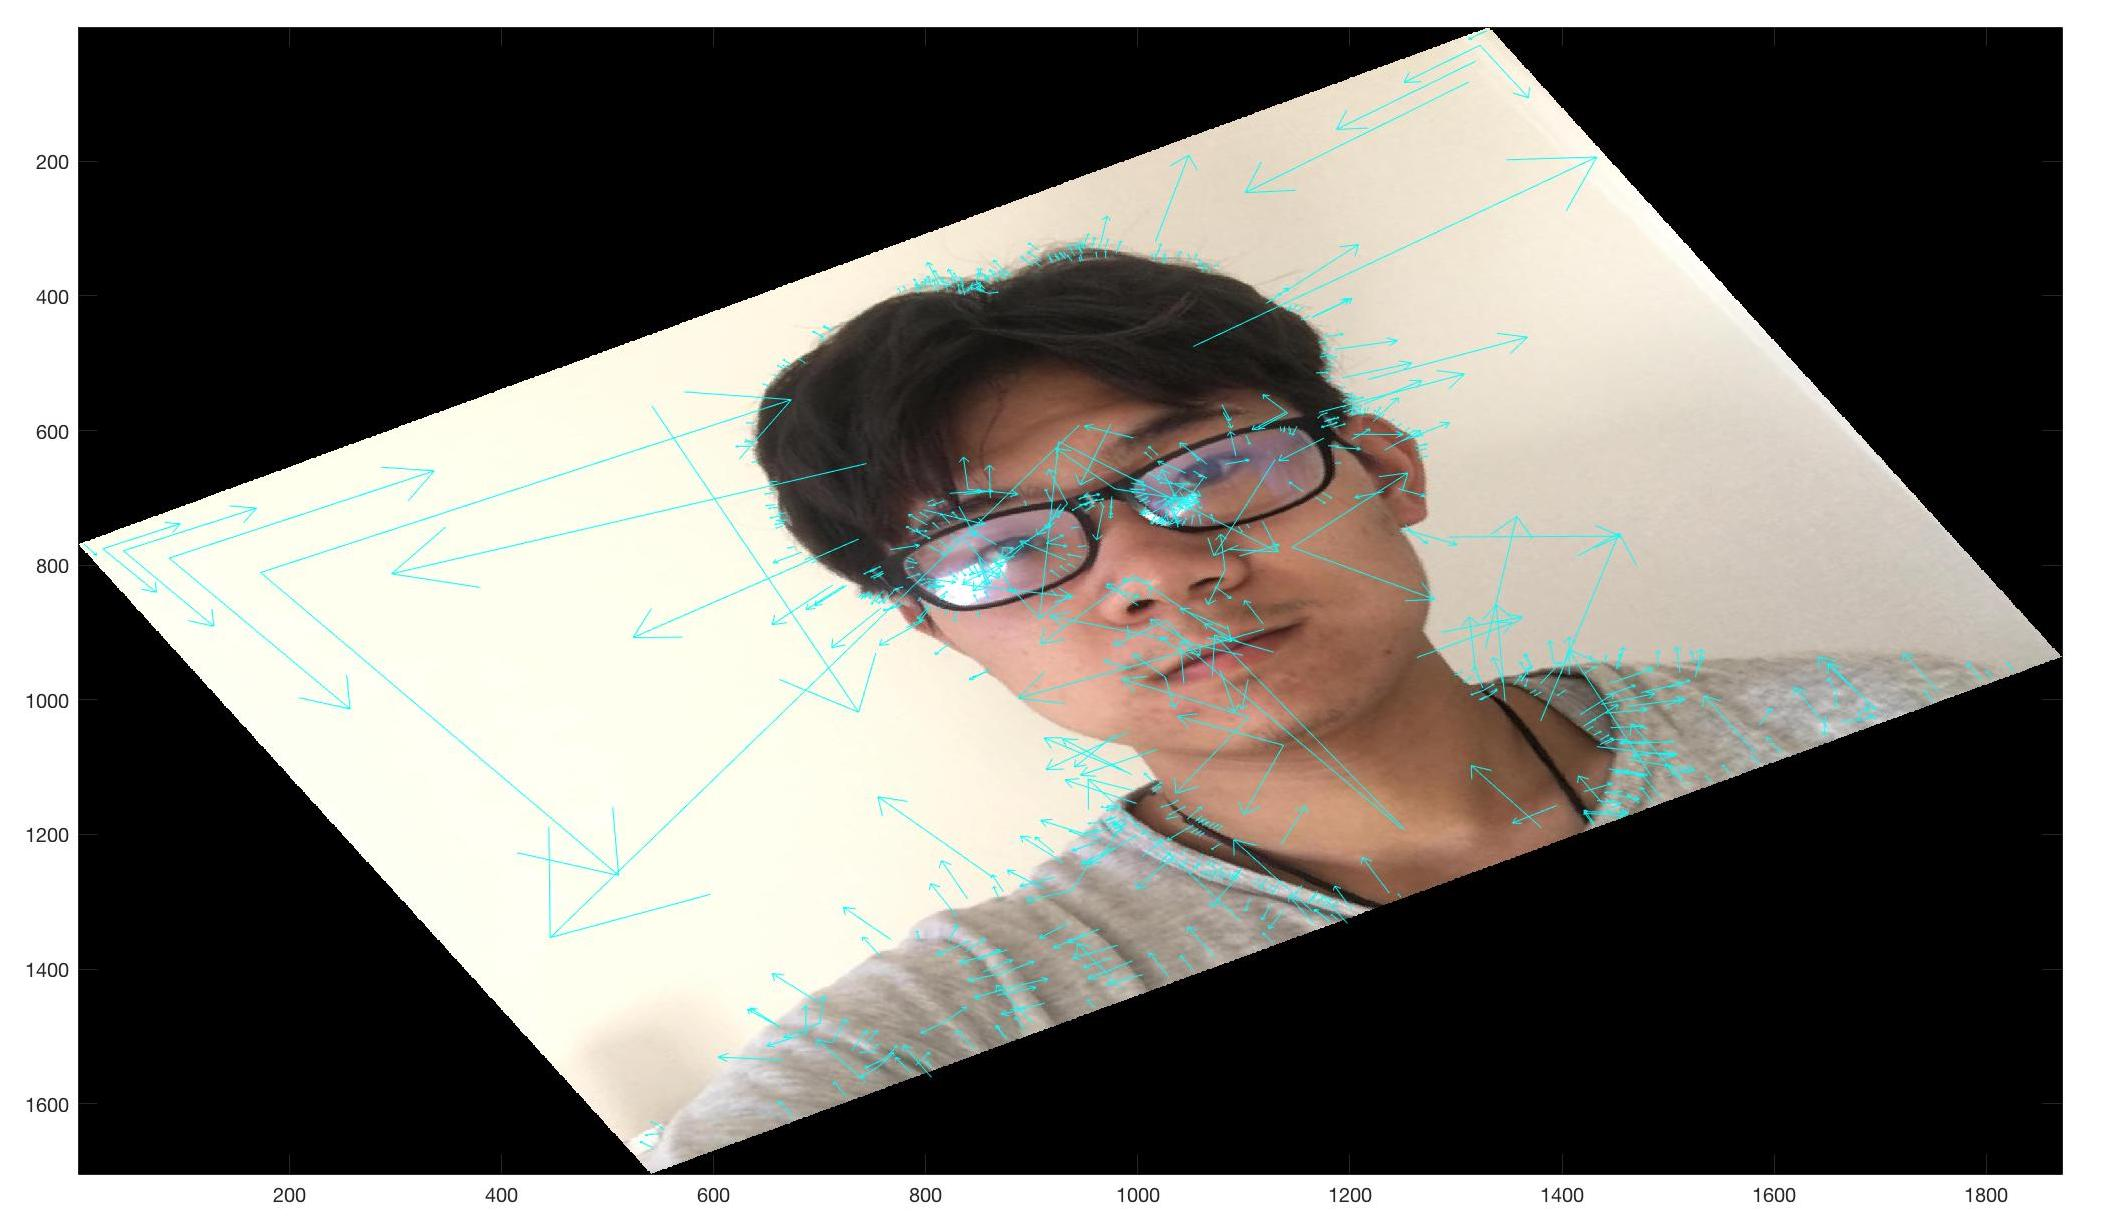
\includegraphics[scale = 0.1]{fig21.jpg}
    \caption{SIFT result of the second processed image.}
    \label{fig21}
\end{figure}

\begin{figure}[htbp]
    \centering
    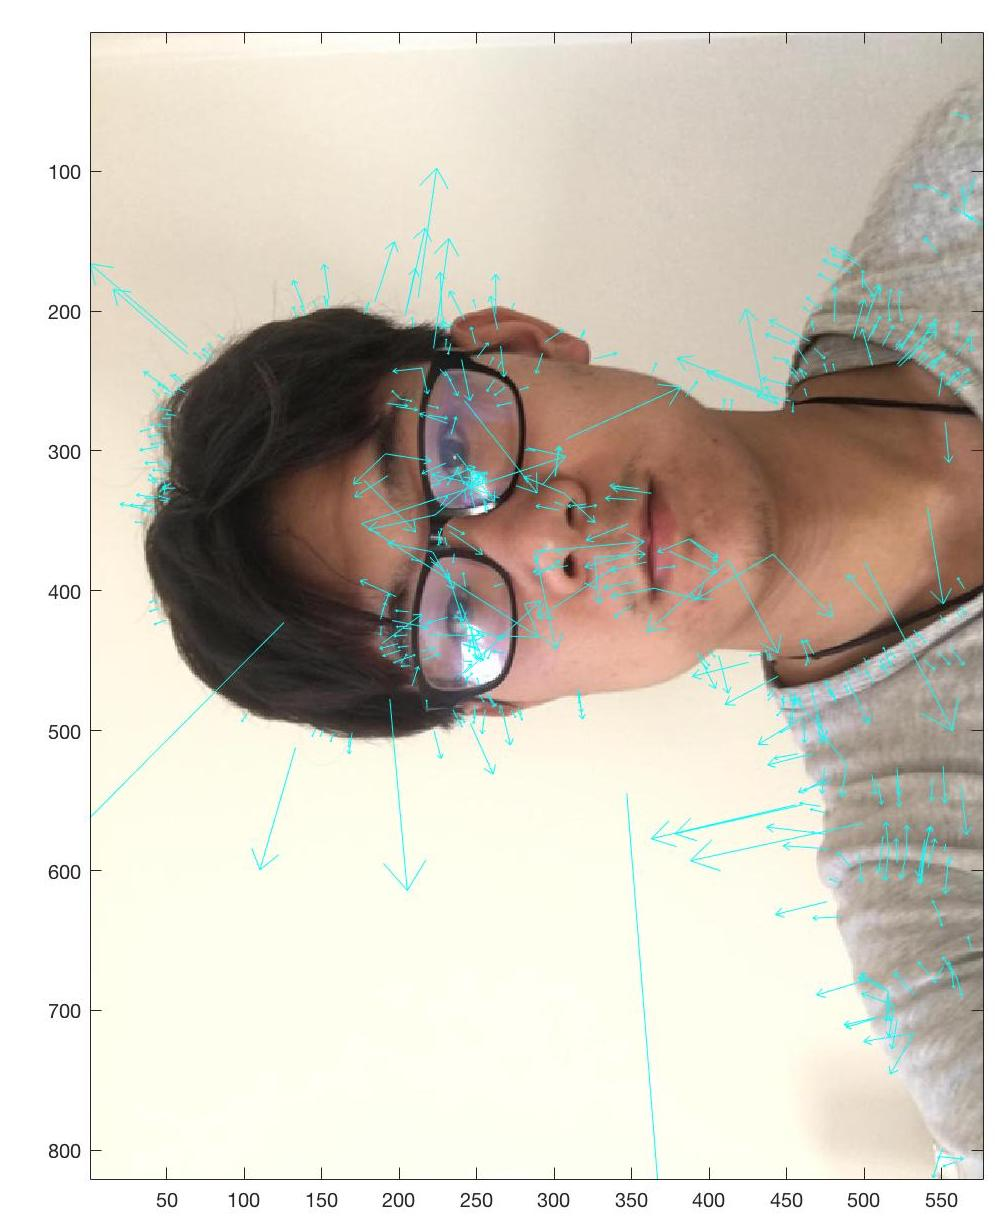
\includegraphics[scale = 0.1]{fig22.jpg}
    \caption{SIFT result of the third processed image.}
    \label{fig22}
\end{figure}

\subsubsection*{Step 3: Display two images, find the SIFT feature points and match them.}

For this subtask, I first choose two images. Let us name them im1 and im2. The algorithm to find the matching points is easy. I just calculate the distance between each two sift point of the two images. If two points are matched, then the distance between them are much too smaller than others. So I conduct the following method:

For each point(vector) in im1, calculate all the distance from it to all the points in im2. Then sort the distance and select the smallest two distances. If the two values are $s_1$ and $s_2$($s_1 < s_2$). Then if $s_1 < k\times s_2$, I assume they are matched. I set k as 0.6 here.

The following codes shows the algorithm:

\begin{lstlisting}
%Step 3: Match features
% Matlab inbuilt function matchFeatures work well for the this problem.
% But I still write my own codes to practice the algorithm.
%
%chosen images: im0 and im3

min_locations = [];
[a0,b0] = size(des_ori);
[a1,b1] = size(des_im3);
k = 0.6;
for i = 1:a0
    orin2im3 = repmat(des_ori(i,:),a1,1);
    %map one line in the original image to a map.
    % like (1,2,3)-->(1,2,3;1,2,3;1,2,3)
    distance = sum((orin2im3 - des_im3).^2,2);
    distance = sqrt(distance);
    sort_distance = sort(distance);
    if sort_distance(1)<k*sort_distance(2)
        min_locations = [min_locations;i,find(distance == sort_distance(1))];
    end
    
end

matchpoints1 = locs0(min_locations(1:10,1),1:2);
matchpoints2 = locs3(min_locations(1:10,2),1:2);


figure;
showMatchedFeatures(fin, im3,[matchpoints1(:,2),matchpoints1(:,1)], [matchpoints2(:,2),matchpoints2(:,1)], 'montage', 'parent',axes);

\end{lstlisting}

Figure 23 shows the matching points from the original image and the third image. It matches well! To test the robustness of the codes, I also test the matching point from image 1 to image 3. Figure 24 shows the result. These two results show that my algorithm is powerful and robust.

\begin{figure}[htbp]
    \centering
    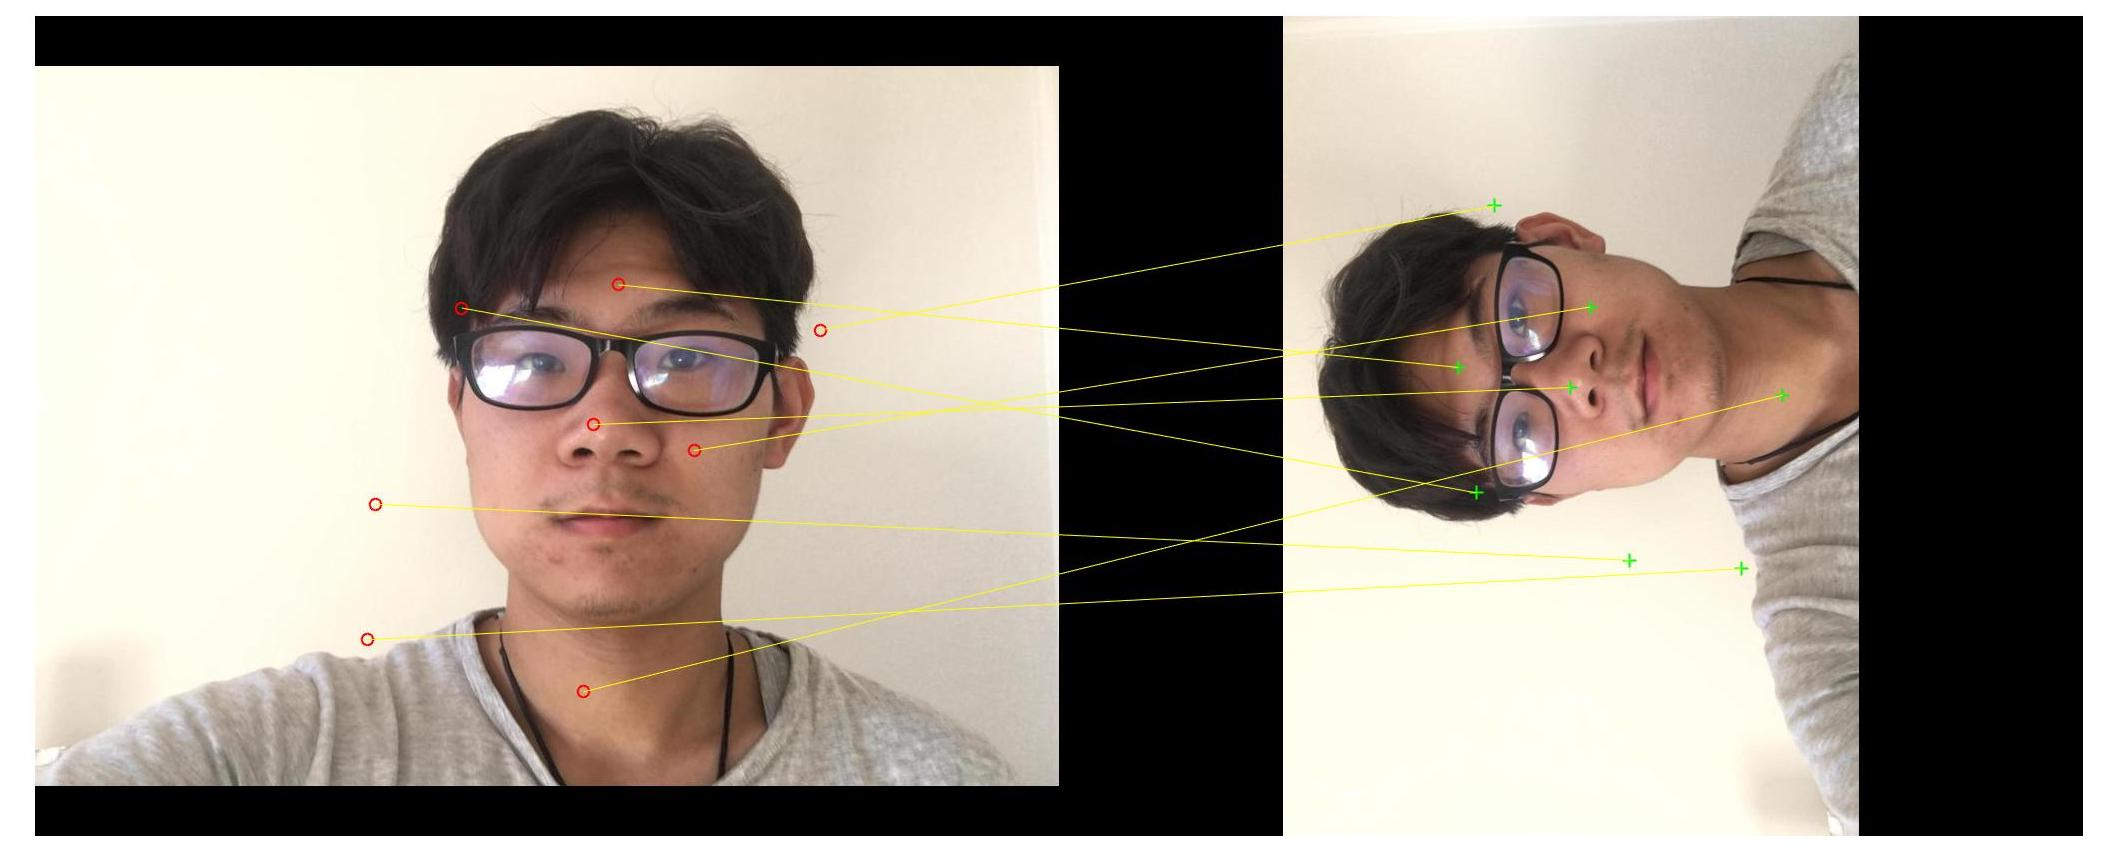
\includegraphics[scale = 0.1]{fig23.jpg}
    \caption{Matching points from original image to image 3.}
    \label{fig23}
\end{figure}

\begin{figure}[htbp]
    \centering
    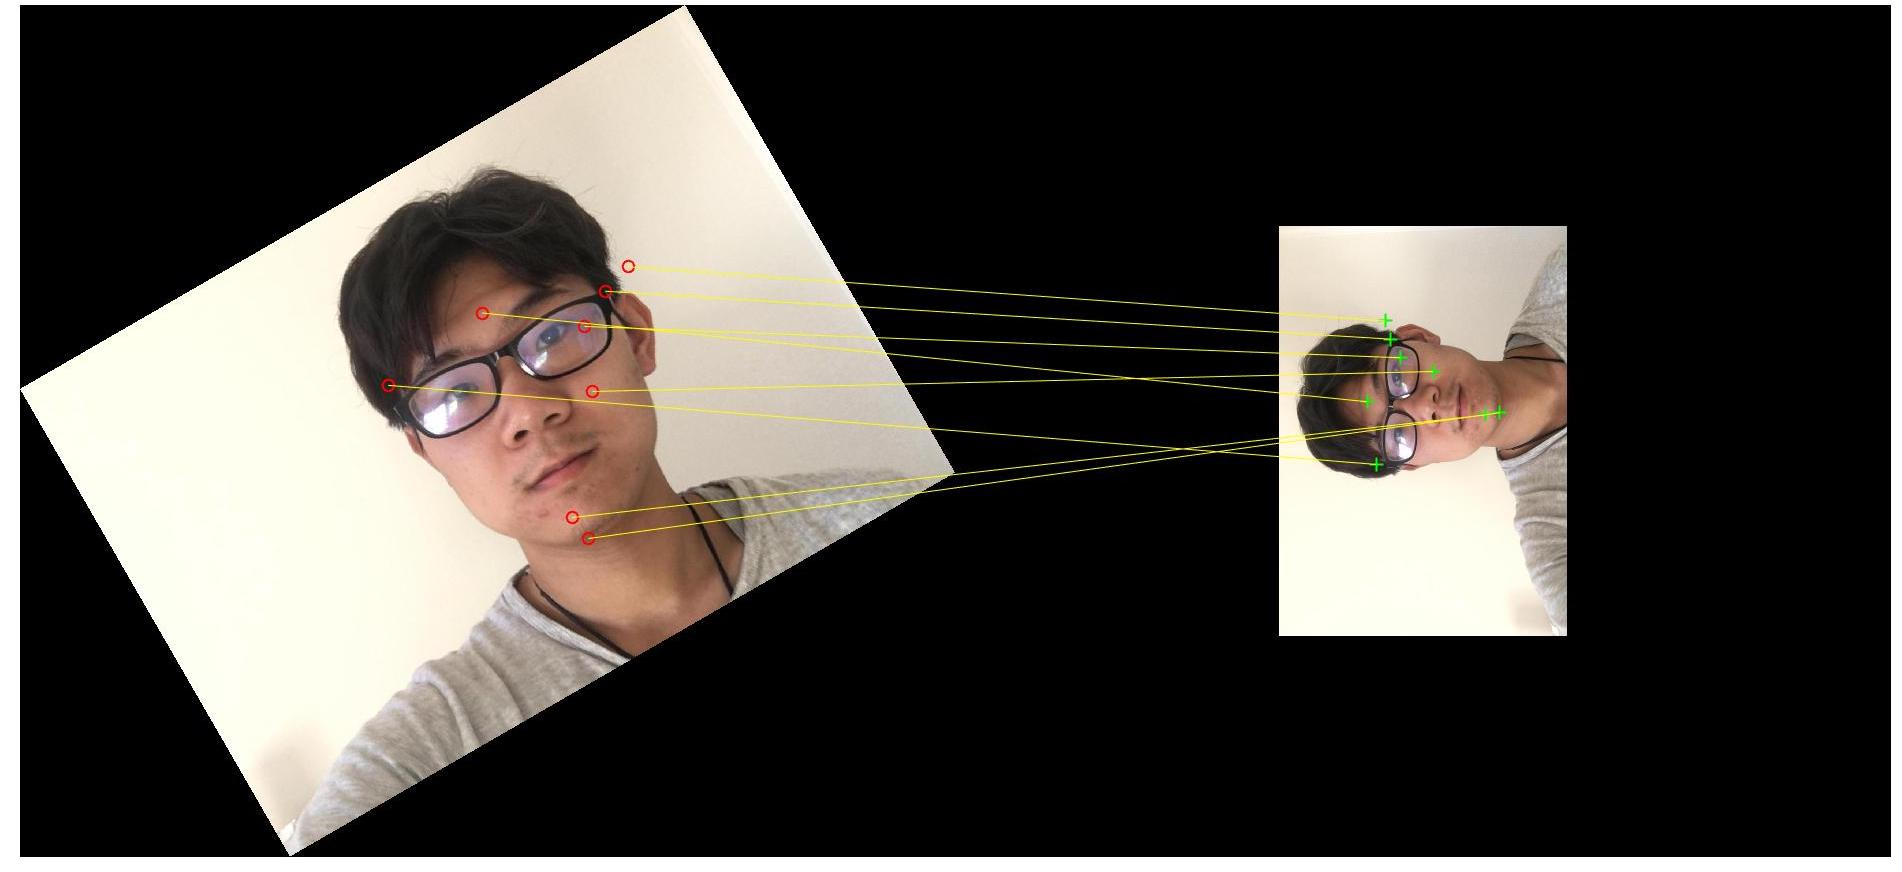
\includegraphics[scale = 0.1]{fig24.jpg}
    \caption{Matching points from image 1 to image 3.}
    \label{fig24}
\end{figure}


\section*{Some other supported codes}
\subsection*{Main codes for task 1:}
\begin{lstlisting}
close all;
clear all;
clc;

im = imread('./images/Lenna.png');
bw = rgb2gray(im);
figure;
subplot(1,2,1);
imshow(bw);

[cols,rws] = my_corner_detector(bw,2,50000000000,11);

hold on;
plot(rws,cols,'or');
title('\bf My Harris Corners with thresh 5e10');

subplot(1,2,2);
imshow(bw);

[cols,rws] = my_corner_detector(bw,2,500000000,11);

hold on;
plot(rws,cols,'or');
title('\bf My Harris Corners with thresh 5e8');


%{
subplot(1,2,2);
imshow(bw);
hold on;
CRNs = corner(bw);
plot(CRNs(:,1),CRNs(:,2),'or');
title('\bf Matlab Harris Corners');
%}

\end{lstlisting}

\subsection*{Main codes for task 2:}
\begin{lstlisting}
clear all;
close all;
clc;

%Step 1: Read input image
path1 = './images/Peppers.png';
img1 = imread(path1);
img1 = uint8(img1/2^8);
%imshow(img1);


path2 = './images/mandm.png';
img1 = imread(path2);
imshow(img1);


title('Input Color Image');

%Step 2: Convert the image to lab channel
cform = makecform('srgb2lab');
lab = applycform(img1,cform);

%Step 3: Form 5-Dimension feature vector.
features = im2feature(lab);

%Step 4: Implement your own k-mean algorithm 

%Step 5: display the segmentation result, by calling the following
%supporting function.
[data_clusters, cluster_stats] = my_kmeans( features, 10 );
displayclusters(lab,data_clusters);

\end{lstlisting}

\subsection*{Whole codes of k-means function for task 2:}
\begin{lstlisting}
function [data_clusters, cluster_stats] = my_kmeans( data, nc )
% This function performs k-means clustering on data 
%given (nc) = the number of clusters.
%  Random Initialization
data = double(data);
ndata = size(data,1);
ndims = size(data,2);

random_labels = floor(rand(ndata,1) * nc) + 1;

data_clusters = random_labels;

cluster_stats = zeros(nc,ndims+1);

distances = zeros(ndata,nc);

while(1)
    
    pause(0.03);
    
    % Make a copy of cluster statistics for 
    % comparison purposes.  If the difference is very small, the while loop will exit.
    last_clusters = cluster_stats;
    
    % For each cluster    
    for c=1:nc
        
        % Find all data points assigned to this cluster
        [ind] = find(data_clusters == c);
        num_assigned = size(ind,1); %number of 
        
        % some heuristic codes for exception handling. 
        if( num_assigned < 1 )
            disp('No points were assigned to this cluster, some special processing is given below');
            
            % Calculate the maximum distances from each cluster
            max_distances = max(distances);
            
            [maxx,cluster_num] = max(max_distances);
            [maxx,data_point] = max(distances(:,cluster_num));
            
            data_clusters(data_point) = cluster_num;
            
            ind = data_point;
            num_assigned = 1;
        end   %% end of exception handling.   
        
        % Save number of points per cluster,  plus the mean vectors.
        cluster_stats(c,1) = num_assigned;
        if( num_assigned > 1 )
            summ = sum(data(ind,:));
            cluster_stats(c,2:ndims+1) = summ / num_assigned;
        else
            cluster_stats(c,2:ndims+1) = data(ind,:);
        end
        
    end
    
    % Exit criteria
    diff = sum(abs(cluster_stats(:) - last_clusters(:)));
    if( diff < 0.00001 )
        break;
    end
    
    % - Set each cluster center to the average of the points assigned to it.
    
    % - calculate the distance from each point to each cluster center.  
    cluster_position = cluster_stats(:,2:end); 
    for i = 1:nc
        a = data-repmat(cluster_position(i,:),ndata,1);
        distances(:,i) = sqrt(sum(a.^2,2));
    end
    
	%%update the membership assignment, i.e., update the data_clusters with current values.  
    for i = 1:ndata
        data_clusters(i) = find(distances(i,:) == min(distances(i,:)),1);
    end
    % Display clusters for the purpose of debugging.  
    %pause;
 end 

\end{lstlisting}

\subsection*{Main codes for task 3:}
\begin{lstlisting}
clear all;
close all;
clc;
%Step 1: read in and rotate images
fin = imread('face_02_u6600985.jpg');
%rotate 30,60,90, rescale: 1.5,1.2,0.8
im1 = imrotate(imresize(fin,1.5),30);
im2 = imrotate(imresize(fin,1.2),60);
im3 = imrotate(imresize(fin,0.8),90);
%show images
figure;
subplot(2,2,1);
imshow(fin);
title('original image');
subplot(2,2,2);
imshow(im1);
title('rotate 30 angles and rescale 1.5');
subplot(2,2,3);
imshow(im2);
title('rotate 60 angles and rescale 1.2');
subplot(2,2,4);
imshow(im3);
title('rotate 90 angles and rescale 0.8');
%save images
imwrite(im1,'im1.jpg');
imwrite(im2,'im2.jpg');
imwrite(im3,'im3.jpg');

%Step 2: show sift images
%draw sift images
[des_ori, locs0] = my_sift(fin,'origin.key');
%showkeys(fin,locs0);
[des_im1, locs1] = my_sift(im1,'im1.key');
%showkeys(im1,locs1);
[des_im2, locs2] = my_sift(im2,'im2.key');
%showkeys(im2,locs2);
[des_im3, locs3] = my_sift(im3,'im3.key');
%showkeys(im3,locs3);

%Step 3: Match features
% Matlab inbuilt function matchFeatures work well for the this problem.
% But I still write my own codes to practice the algorithm.
%
%chosen images: im0 and im3

min_locations = [];
[a0,b0] = size(des_ori);
[a1,b1] = size(des_im3);
k = 0.6;
for i = 1:a0
    orin2im3 = repmat(des_ori(i,:),a1,1);
    %map one line in the original image to a map.
    % like (1,2,3)-->(1,2,3;1,2,3;1,2,3)
    distance = sum((orin2im3 - des_im3).^2,2);
    distance = sqrt(distance);
    sort_distance = sort(distance);
    if sort_distance(1)<k*sort_distance(2)
        min_locations = [min_locations;i,find(distance == sort_distance(1))];
    end
    
end

matchpoints1 = locs0(min_locations(1:10,1),1:2);
matchpoints2 = locs3(min_locations(1:10,2),1:2);


figure;
showMatchedFeatures(fin, im3,[matchpoints1(:,2),matchpoints1(:,1)], [matchpoints2(:,2),matchpoints2(:,1)], 'montage', 'parent',axes);

\end{lstlisting}

\end{document}


